\section{Out-of-sample embedding}
\label{sec:ch7:oos}

While the networks that we have been using in this book have generally been on the small side, for larger networks, computing embeddings can be expensive. In Remark \ref{box:ch7:oos:ex}, we detail an example of why this is the case.

\begin{floatingbox}[h]\caption{Spectral embeddings of networks with many nodes}
\label{box:ch7:oos:ex}
Let's imagine that you have a network, where the nodes are web pages and the edges are whether a pair of web pages cross-link to one another. There are $n=10^9$ nodes in the network, and let's imagine that you have a strong suspicion that there are communities that are homophilic (they have high within-community clustering). For any given day, you want to have a record of the estimated communities that exist in your network. Procedurally, we learned how to address this task in Section \ref{sec:ch7:comm_detect}: you begin by embedding the network, and then you train an unsupervised classifier to identify estimated community structure from the estimated latent positions.

The next day, however, you have a problem: another $n'=5$ web pages were added to the network. Being a diligent machine learning scientist, you could simply re-execute your procedure you used the previous day. However, this has a limitation: the \texttt{svd} (a crucial component of spectral embeddings), while more than sufficient for the networks that we have been working with in this book, does not scale particularly well to large networks. The \textit{time complexity} refers to the amount of time that it takes an algorithm (in the worst case) to yield a solution, and the \textit{space complexity} refers to the amount of RAM that the computer would need to access to yield a solution. When working with large networks and using complicated algorithms, the time and space complexity will be problems that we will need to contend with. If you are unfamiliar with time and space complexity, we would recommend that you review \cite{Banerjee2021Dec}.

The \texttt{svd} tends to scale in $\mathcal O(n^3)$ time, and the space requirements are no better, scaling at about $\mathcal O(n^2)$. This means that for networks with more nodes, embedding the network will take a lot of computing time and space to calculate. Your web pages network is very large, so this could get expensive very quickly!
\end{floatingbox}

The key problem is that the network is extremely large, and the \texttt{svd} (and consequently, the \texttt{ase}) scales remarkably poorly for large networks. When you embed large networks, you might have to resort to using special super computers with enormous numbers of cores or memory to get the results that you need. These computers tend to be expensive, so the cost of this operation could skyrocket quickly. 

Remember that when we make assumptions that our network $A$ is a sample from an underlying random network $\mathbf A$ as in Section \ref{sec:ch6:ase:whyuse}, the estimates of latent positions produced by \texttt{ase} tend to be fairly close estimates of the true underlying latent positions in the network. Further, as the network grows, these estimates get better and better. This means that if we embedded a network with $n + n'$ nodes, the embedding is probably going to be fractionally better than the embedding if we just used $n$ nodes. 

The difference, however, will not be particularly substantial, and sometimes we might be willing to take a slight loss in the precision of our estimates at the tradeoff of having far greater computational and algorithmic efficiency. In these cases, we can use an \textit{out of sample embedding}, or \texttt{oose} \cite{Levin2018Jul,Bengio2003}, to embed new nodes (the ``out-of-sample'' nodes) in an existing latent space computed using only the original nodes (the ``in-sample'' nodes). 

When we do this, we obtain estimated latent positions for our new nodes in a shared space between the new and old nodes. While we might still want to recompute the full embedding occassionally, in the short term we can save a lot of computation resources (which can mean time, money, and effort) and still obtain estimated latent positions that are good enough for our downstream analysis.

\subsection{\texttt{oose} requires a full adjacency matrix and adjacency vectors for each new node}

Let's begin by generating a network. For the out-of-sample embedding, we first need an $n$-node network (the ``in-sample'' nodes). The crucial ingredient that we will need for the out-of-sample nodes are instructions that tell us how the out-of-sample nodes are connected to the ``in-sample'' nodes. This is accomplished via adjacency vectors, which can be thought of as behaving a lot like ``rows'' of an adjacency matrix. An \textit{adjacency vector} for a node $j$ in relation to an $n$-node network is a length-$n$ vector $\vec a_j$, where $a_{ij}$ indicates whether node $i$ and node $j$ are connected.

For demonstration purposes, we'll generate a sample from an $SBM_n(\vec z, B)$ random network with $n + n'$ nodes. The in-sample nodes will be $50$ nodes from community $1$, and $50$ nodes from community $2$. The out-of-sample nodes will be $1$ node from community $1$, and $2$ nodes from community $2$:

\begin{lstlisting}[style=python]
import numpy as np
from graspologic.simulations import sbm

# the in-sample nodes
n = 100
nk = 50
# the out-of-sample nodes
np1 = 1; np2 = 2
B = np.array([[0.6, 0.2], [0.2, 0.4]])
# sample network
A, zs = sbm([nk + np1, nk + np2], B, return_labels=True)
\end{lstlisting}

Next, we will remove the $n'$ ``out-of-sample'' nodes with \texttt{graspologic}. This will give us an $n \times n$ adjacency matrix corresponding to the subnetwork induced by the in-sample nodes, and an $n \times n'$ matrix $A'$ of adjacency vectors, which indicate the connectivity of out-of-sample nodes to in-sample nodes:

\begin{lstlisting}[style=python]
from graspologic.utils import remove_vertices

# the indices of the out-of-sample nodes
oos_idx = [nk, nk + np1 + nk, nk + np1 + nk + 1]
# get adjacency matrix and the adjacency vectors A prime
Ain, Ap = remove_vertices(A, indices=oos_idx, return_removed=True)
\end{lstlisting}

In Figure \ref{fig:ch7:oos:ex}(A), we plot the adjacency matrix of the in-sample nodes. Note the modular community structure. In Figure \ref{fig:ch7:oos:ex}(B), we show the adjacency vectors for each of the $3$ out-of-sample nodes, in relation to the in-sample nodes from Figure \ref{fig:ch7:oos:ex}(A). Further, notice that the out-of-sample nodes tend to follow the patterns from their respective communities; out-of-sample node $1$ is in community $1$, and tends to have more connections with nodes of community $1$. Out-of-sample nodes $2$ and $3$ are in community $2$, and tend to have more connections with nodes of community $2$.

\begin{figure}[h]
    \centering
    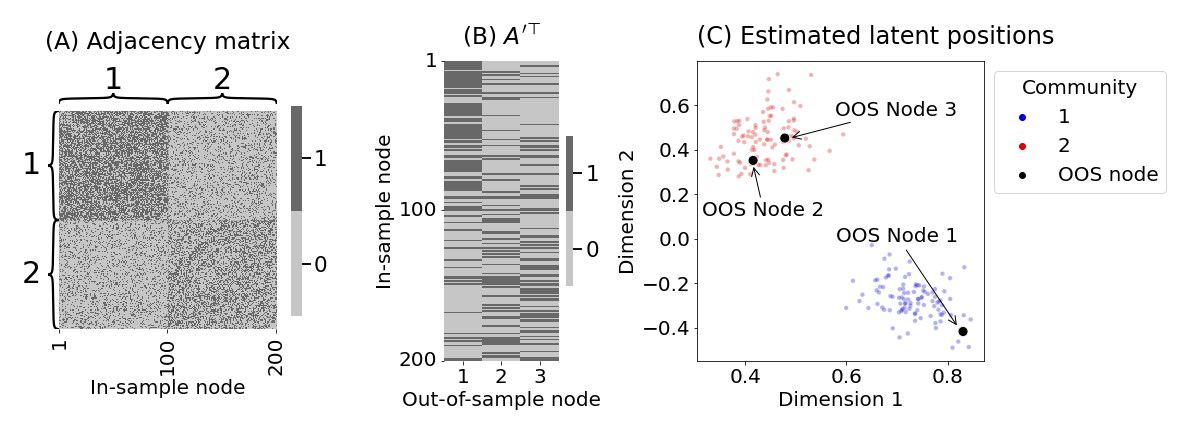
\includegraphics[width=\linewidth]{applications/ch7/Images/oos_ex.png}
    \caption[Out of sample embedding example]{\textbf{(A)} the adjacency matrix for the in-sample nodes. \textbf{(B)} the adjacency vectors (columns) for each of the $3$ out-of-sample nodes. \textbf{(C)} the estimated latent positions for each of the in-sample nodes (faint blue and red) with the estimated latent positions for the out-of-sample nodes (black).}
    \label{fig:ch7:oos:ex}
\end{figure}

\subsection{Conceptualizing the probability vector for an out-of-sample node}

If we add an out-of-sample node $j$ to the network, the adjacency matrix for this new network is:
\begin{align*}
    A &= \begin{bmatrix}
        A & \vec a_j \\
        \vec a_j^\top & 0
    \end{bmatrix}
\end{align*}

Where the $j$ simply denotes that we added the node $j$ to the network, and $\vec a_j$ is the adjacency vector for node $j$. If we assume that this new network is a sample from an $RDPG_{n+1}(X')$ random network, the latent position matrix is:
\begin{align*}
    X' &= \begin{bmatrix}
        \vec x_1^\top \\
        \vdots\\
        \vec x_n^\top \\
        \vec x_j^\top
    \end{bmatrix}
\end{align*}
where $\vec x_j$ is the latent position (the quantity that we want to obtain) associated with our out-of-sample node $j$.

Remember that for an $RDPG_{n+1}(X')$ random network, that for all pairs of nodes $i$ and $i'$, $p_{ii'} = \vec x_i^\top \vec x_{i'}$. Therefore, the matrix product $X\vec x_j$ is:
\begin{align*}
    X\vec x_j &= \begin{bmatrix}
        \vec x_1^\top \\
        \vdots \\
        \vec x_n^\top
    \end{bmatrix}\vec x_j = \begin{bmatrix}
        \vec x_1^\top \vec x_j \\
        \vdots \\
        \vec x_n^\top \vec x_j
    \end{bmatrix} = \begin{bmatrix}
        p_{1j} \\
        \vdots \\
        p_{nj}
    \end{bmatrix} = \vec p_{j},
\end{align*}
where we just used the standard rules of matrix multiplication for the second equality, and then used the definition of $p_{ij}$ for the in-sample nodes. We will call this vector $\vec p_{j}$ the probability vector of node $j$, which has entries $p_{ij}$ for all $n$ in-sample nodes. In particular, this implies that:
\begin{align*}
    X\vec x_j - \vec p_{j} = \vec 0 = \begin{bmatrix}
        0 \\
        \vdots \\
        0 
    \end{bmatrix}, \numberthis \label{eqn:ch7:oos:e1}
\end{align*}
where $\vec 0$ is the $n$-dimensional $0$ vector.

\subsection{Estimating the out-of-sample node's latent position}

Our goal is to obtain an estimate of $\vec x_j$. Note that in Equation \ref{eqn:ch7:oos:e1}, we have two unobserved quantities here, $X$ and $\vec p_j$ (the probability vector for the node $j$). 

\subsubsection*{Estimating the unobserved quantities}

\paragraph*{Estimating the latent positions of the in-sample nodes}
Under our given setup, if $\mathbf A$ is a random network, it's not much of a stretch to assume that the network of only the in-sample nodes is an $RDPG_n(X)$ random network. By the logic that we developed in Section \ref{sec:ch6:ase}, a reasonable approach would be to use the \texttt{ase} to estimate latent positions for the in-sample nodes. We can do this using \texttt{graspologic}, with:

\begin{lstlisting}[style=python]
from graspologic.embed import AdjacencySpectralEmbed as ase

oos_embedder = ase()
# estimate latent positions for the in-sample nodes
# using the subnetwork induced by the in-sample nodes
Xhat_in = oos_embedder.fit_transform(Ain)
\end{lstlisting}

The in-sample estimated latent positions are shown in Figure \ref{fig:ch7:oos:ex}(C), with the faint colored nodes. The estimated latent positions are as-described for the estimated latent positions of a two-community $SBM_n(\vec z, B)$ random network: two relatively homogeneous (in terms of the latent positions) clusters of nodes. Remember that this is a function of the fact that the latent positions for a $SBM_n(\vec z, B)$ random network are identical within-community as-per Section \ref{sec:ch5:psd_block:same_lp}, and the estimated latent positions are estimating the latent positions.

\paragraph*{Formulating a least-squares optimization problem to estimate the probability vector}

Next, we'll turn to estimating $\vec p_j$.

\begin{floatingbox}[h]\caption{Estimating probabilities}
\label{box:ch7:oos:probs}
In section \ref{sec:ch6:mle}, we covered a basic result from probability for finding maximum likelihood estimates for coin flips. Let's assume that you have a random coin $\mathbf y$. For our purposes, let's imagine that this coin lands on heads (a value of $1$) with probability $p$ and tails (a value of $0$) with probability $1 - p$.

If you flip the coin $m$ times and obtain samples of coin flips $y_i$, a reasonable estimate of the probability that the coin lands on heads is given by the maximum likelihood estimate (MLE):
\begin{align*}
    \hat p &= \frac{1}{m}\sum_{i = 1}^m y_i,
\end{align*}
which is simply the fraction of the $m$ coin flips that landed on heads. 
\end{floatingbox}

As a logical extension of Remark \ref{box:ch7:oos:probs}, if you had one coin flip, the MLE would just be the outcome of that coin flip. With an identical rationale, we estimate $\vec p_j$ using:
\begin{align*}
    \hat p_{ij} &= a_{ij}.
\end{align*}
We estimate the probability that the in-sample nodes nodes $i$ and the out-of-sample node $j$ are connected as the adjacency value $a_{ij}$ between them. Stated another way, we will estimate $\hat{\vec p}_j$ with $\vec a_j$.

$\hat X$ is only an estimate of $X$, and is also inexact, which you learned about in Section \ref{sec:ch6:ase:whyuse}. Likewise, it is extremely unlikely that $\hat p_{ij} = p_{ij}$; that is, estimating the probability that the in-sample node $i$ and the out-of-sample node $j$ are connected with a single observation from the adjacency vector is probably not going to give us a particularly exact solution.  

Next, we're going to use what we have established in Equation \eqref{eqn:ch7:oos:e1} to establish a least-squares optimization problem. You can read about least-squares regression in Remark \ref{box:ch7:oos:lsreg} for a quick refresher. For a more detailed overview, check out \cite{Geron2017Mar}.

\begin{floatingbox}[h]\caption{Ordinary least-squares (OLS) regression}
\label{box:ch7:oos:lsreg}
Through least squares regression, you observe $n$ samples $y_i$, along with a set of features $\vec x_i$, which is a $d$-dimensional feature vector for each sample $i$. Your goal is to identify a set of $d$ coefficients $\vec \beta$, where for all $n$ samples:
\begin{align*}
    \vec y = \begin{bmatrix}
        y_1 \\
        \vdots \\
        y_n
    \end{bmatrix}&= X \vec \beta = \begin{bmatrix}
        \leftarrow & \vec x_1^\top & \rightarrow \\
        & \vdots &  \\
        \leftarrow & \vec x_n^\top & \rightarrow 
    \end{bmatrix}\begin{bmatrix}
        \beta_1 \\
        \vdots \\
        \beta_d
    \end{bmatrix}.
\end{align*}
By subtracting $X\beta$ from both sides, we obtain that:
\begin{align*}
    \vec y - X\vec\beta &= \vec 0,
\end{align*}
Unfortunately, the samples are noisy in practice, So we are limited to getting a close approximation of each sample; e.g.:
\begin{align*}
    y_i - \vec x_i^\top \beta &= r_i,\text{ and consequently, }\vec y - X\beta = \vec r
\end{align*}
where $r_i$ is known as the residual or error associated with sample $i$ in the regression. The \textit{mean-squared error} is defined as:
\begin{align*}
    MSE(\vec \beta) &= \frac{1}{n}\sum_{i = 1}^n\left(r_i\right)^2 = \frac{1}{n}\|X\vec \beta - \vec y\|^2_2.
\end{align*}
Our goal is to find the choice of $\vec \beta$ that minimizes the mean-squared error. With a bit of calculus, the solution to this is given by the \textit{normal equations}:
\begin{align*}
    \hat{\vec \beta} &= (X^\top X)^{-1}X^\top \vec y.
\end{align*}
\end{floatingbox}

Since our estimates of $X$ via $\hat X$ and $\vec p_j$ via $\vec a_j$ are imperfect, when we plug these into Equation \ref{eqn:ch7:oos:e1}, our equation becomes:
\begin{align*}
    \hat X \vec x_j - \vec a_j = \vec e_j,
\end{align*}
where $\vec e_j$ is an $n$-dimensional error term. In an ideal world, $\vec e_j$ would be exactly the zero vector, but since we imperfectly estimated $X$ and $\vec p_j$ with $\hat X$ and $\vec a_j$, this will not be the case. For this reason, we turn to least-squares regression. 

Using the normal equations in Remark \ref{box:ch7:oos:lsreg}, the estimate of $\vec x_j$ that minimizes the mean-squared error is given by:
\begin{align*}
    \hat{\vec x}_j &= \left(\hat X^\top \hat X\right)^{-1}\hat X^\top \vec a_j.\numberthis \label{eqn:ch7:oos:lsoose}
\end{align*}
This estimate $\hat{\vec x}_j$ is known as the \textit{least squares out-of-sample embedding} the out-of-sample node $j$. 

In the general case when you have $n'$ out-of-sample nodes with adjacency vectors to the in-sample nodes, the least-squares out-of-sample embedding (least-squares \texttt{oose}) for the out-of-sample nodes can be found using the procedure in Algorithm \ref{alg:ch7:oose}.

\begin{algorithm}
\label{alg:ch7:oose}
\caption{Least-squares out-of-sample embedding (least-squares \texttt{oose})}
\KwData{An estimated latent position matrix $\hat X$ for the in-sample nodes. \newline
$A'$, wich is a $n \times n'$ matrix whose columns $\vec a_j$ indicate the adjacency vectors $\vec a_j$ for each of the $n'$ out-of-sample nodes with the in-sample nodes.}
\KwResult{$d \times n'$ matrix, whose columns indicate the estimated latent positions for each of the $n'$ out-of-sample nodes.}
\SetAlgoLined

Let $\hat X' = \left(\hat X^\top \hat X\right)^{-1}\hat X^\top A'$.

\Return{$\hat X'$}
\end{algorithm}

We can perform embed the least-squares \texttt{oose} using \texttt{graspologic}:

\begin{lstlisting}[style=python]
Xhat_oos = oos_embedder.transform(Ap)
\end{lstlisting}
The embedding for the out-of-sample nodes is shown in Figure \ref{fig:ch7:oos:ex}(C). Note that out-of-sample node $1$ was in community $1$, and has an estimated latent position near those of the in-sample nodes from community $1$. Likewise, the out-of-sample nodes $2$ and $3$ were in community $2$, and have estimated latent positions near the in-sample nodes from community $2$. In this sense, least-squares \texttt{oose} has preserved the relative homogeneity in the latent positions within-community for the out-of-sample nodes with respect to the in-sample nodes, without requiring the in-sample network to be re-embedded.

\subsection{Computational Considerations}

Adapting the result from Remark \ref{box:ch7:oos:ex}, the spectral embeddings require the \texttt{svd} for the new network with $n + n'$ nodes where the number of in-sample nodes $n$ greatly exceeds the number of out-of-sample nodes $n'$. The time complexity of the \texttt{svd} is $\mathcal O\left(n^3\right)$, and the space complexity is $\mathcal O\left(n^2\right)$. 

On the other hand, the least-squares solution in Algorithm \ref{alg:ch7:oose} has a time complexity of $\mathcal O\left(d^2 n\right)$. If the embedding is meaningful, the number of estimated latent dimensions is usually far less than the number of nodes. So this approach has far improved time scalability over re-embedding the entire network, because for networks with large numbers of nodes $n^3$ will be much larger than $d^2 n$.

Space wise, when the number of in-sample nodes exceeds the number of estimated latent dimensions and the number of out-of-sample nodes, the space complexity to solve the normal equations is $\mathcal O\left(dn\right)$. By the same logic as above, $dn$ is much less than $n^2$, so the normal equations can be solved with far less space than recomputing the embedding.

\newpage